\PassOptionsToPackage{unicode=true}{hyperref} % options for packages loaded elsewhere
\PassOptionsToPackage{hyphens}{url}
%
\documentclass[ignorenonframetext,]{beamer}
\usepackage{pgfpages}
\setbeamertemplate{caption}[numbered]
\setbeamertemplate{caption label separator}{: }
\setbeamercolor{caption name}{fg=normal text.fg}
\beamertemplatenavigationsymbolsempty
% Prevent slide breaks in the middle of a paragraph:
\widowpenalties 1 10000
\raggedbottom
\setbeamertemplate{part page}{
\centering
\begin{beamercolorbox}[sep=16pt,center]{part title}
  \usebeamerfont{part title}\insertpart\par
\end{beamercolorbox}
}
\setbeamertemplate{section page}{
\centering
\begin{beamercolorbox}[sep=12pt,center]{part title}
  \usebeamerfont{section title}\insertsection\par
\end{beamercolorbox}
}
\setbeamertemplate{subsection page}{
\centering
\begin{beamercolorbox}[sep=8pt,center]{part title}
  \usebeamerfont{subsection title}\insertsubsection\par
\end{beamercolorbox}
}
\AtBeginPart{
  \frame{\partpage}
}
\AtBeginSection{
  \ifbibliography
  \else
    \frame{\sectionpage}
  \fi
}
\AtBeginSubsection{
  \frame{\subsectionpage}
}
\usepackage{lmodern}
\usepackage{amssymb,amsmath}
\usepackage{ifxetex,ifluatex}
\usepackage{fixltx2e} % provides \textsubscript
\ifnum 0\ifxetex 1\fi\ifluatex 1\fi=0 % if pdftex
  \usepackage[T1]{fontenc}
  \usepackage[utf8]{inputenc}
  \usepackage{textcomp} % provides euro and other symbols
\else % if luatex or xelatex
  \usepackage{unicode-math}
  \defaultfontfeatures{Ligatures=TeX,Scale=MatchLowercase}
\fi
% use upquote if available, for straight quotes in verbatim environments
\IfFileExists{upquote.sty}{\usepackage{upquote}}{}
% use microtype if available
\IfFileExists{microtype.sty}{%
\usepackage[]{microtype}
\UseMicrotypeSet[protrusion]{basicmath} % disable protrusion for tt fonts
}{}
\IfFileExists{parskip.sty}{%
\usepackage{parskip}
}{% else
\setlength{\parindent}{0pt}
\setlength{\parskip}{6pt plus 2pt minus 1pt}
}
\usepackage{hyperref}
\hypersetup{
            pdftitle={Simulations de variables aléatoires},
            pdfauthor={Pierre Gloaguen},
            pdfborder={0 0 0},
            breaklinks=true}
\urlstyle{same}  % don't use monospace font for urls
\newif\ifbibliography
\usepackage{color}
\usepackage{fancyvrb}
\newcommand{\VerbBar}{|}
\newcommand{\VERB}{\Verb[commandchars=\\\{\}]}
\DefineVerbatimEnvironment{Highlighting}{Verbatim}{commandchars=\\\{\}}
% Add ',fontsize=\small' for more characters per line
\usepackage{framed}
\definecolor{shadecolor}{RGB}{248,248,248}
\newenvironment{Shaded}{\begin{snugshade}}{\end{snugshade}}
\newcommand{\AlertTok}[1]{\textcolor[rgb]{0.94,0.16,0.16}{#1}}
\newcommand{\AnnotationTok}[1]{\textcolor[rgb]{0.56,0.35,0.01}{\textbf{\textit{#1}}}}
\newcommand{\AttributeTok}[1]{\textcolor[rgb]{0.77,0.63,0.00}{#1}}
\newcommand{\BaseNTok}[1]{\textcolor[rgb]{0.00,0.00,0.81}{#1}}
\newcommand{\BuiltInTok}[1]{#1}
\newcommand{\CharTok}[1]{\textcolor[rgb]{0.31,0.60,0.02}{#1}}
\newcommand{\CommentTok}[1]{\textcolor[rgb]{0.56,0.35,0.01}{\textit{#1}}}
\newcommand{\CommentVarTok}[1]{\textcolor[rgb]{0.56,0.35,0.01}{\textbf{\textit{#1}}}}
\newcommand{\ConstantTok}[1]{\textcolor[rgb]{0.00,0.00,0.00}{#1}}
\newcommand{\ControlFlowTok}[1]{\textcolor[rgb]{0.13,0.29,0.53}{\textbf{#1}}}
\newcommand{\DataTypeTok}[1]{\textcolor[rgb]{0.13,0.29,0.53}{#1}}
\newcommand{\DecValTok}[1]{\textcolor[rgb]{0.00,0.00,0.81}{#1}}
\newcommand{\DocumentationTok}[1]{\textcolor[rgb]{0.56,0.35,0.01}{\textbf{\textit{#1}}}}
\newcommand{\ErrorTok}[1]{\textcolor[rgb]{0.64,0.00,0.00}{\textbf{#1}}}
\newcommand{\ExtensionTok}[1]{#1}
\newcommand{\FloatTok}[1]{\textcolor[rgb]{0.00,0.00,0.81}{#1}}
\newcommand{\FunctionTok}[1]{\textcolor[rgb]{0.00,0.00,0.00}{#1}}
\newcommand{\ImportTok}[1]{#1}
\newcommand{\InformationTok}[1]{\textcolor[rgb]{0.56,0.35,0.01}{\textbf{\textit{#1}}}}
\newcommand{\KeywordTok}[1]{\textcolor[rgb]{0.13,0.29,0.53}{\textbf{#1}}}
\newcommand{\NormalTok}[1]{#1}
\newcommand{\OperatorTok}[1]{\textcolor[rgb]{0.81,0.36,0.00}{\textbf{#1}}}
\newcommand{\OtherTok}[1]{\textcolor[rgb]{0.56,0.35,0.01}{#1}}
\newcommand{\PreprocessorTok}[1]{\textcolor[rgb]{0.56,0.35,0.01}{\textit{#1}}}
\newcommand{\RegionMarkerTok}[1]{#1}
\newcommand{\SpecialCharTok}[1]{\textcolor[rgb]{0.00,0.00,0.00}{#1}}
\newcommand{\SpecialStringTok}[1]{\textcolor[rgb]{0.31,0.60,0.02}{#1}}
\newcommand{\StringTok}[1]{\textcolor[rgb]{0.31,0.60,0.02}{#1}}
\newcommand{\VariableTok}[1]{\textcolor[rgb]{0.00,0.00,0.00}{#1}}
\newcommand{\VerbatimStringTok}[1]{\textcolor[rgb]{0.31,0.60,0.02}{#1}}
\newcommand{\WarningTok}[1]{\textcolor[rgb]{0.56,0.35,0.01}{\textbf{\textit{#1}}}}
\usepackage{graphicx,grffile}
\makeatletter
\def\maxwidth{\ifdim\Gin@nat@width>\linewidth\linewidth\else\Gin@nat@width\fi}
\def\maxheight{\ifdim\Gin@nat@height>\textheight\textheight\else\Gin@nat@height\fi}
\makeatother
% Scale images if necessary, so that they will not overflow the page
% margins by default, and it is still possible to overwrite the defaults
% using explicit options in \includegraphics[width, height, ...]{}
\setkeys{Gin}{width=\maxwidth,height=\maxheight,keepaspectratio}
\setlength{\emergencystretch}{3em}  % prevent overfull lines
\providecommand{\tightlist}{%
  \setlength{\itemsep}{0pt}\setlength{\parskip}{0pt}}
\setcounter{secnumdepth}{0}

% set default figure placement to htbp
\makeatletter
\def\fps@figure{htbp}
\makeatother

\newcommand{\rmd}{\text{d}}
\newcommand{\R}{\mathbb{R}}
\newcommand{\E}{\mathbb{E}}
\newcommand{\V}{\mathbb{V}}
\newcommand{\Unif}{\mathcal{U}}
\newcommand{\Pro}{\mathbb{P}}
\newcommand{\N}{\mathbb{N}}
\newcommand{\Nor}{\mathcal{N}}
\newcommand{\Cov}{\mathbb{C}\text{ov}}
\newcommand{\I}[1]{\mathbf{1}_{#1}}
\newcommand{\e}[1]{\text{e}^{#1}}
\newcommand{\K}{\mathcal{K}}
\newcommand{\seqN}[1]{\left(#1_n\right)_{n\in\N}}
\makeatletter
\let\save@measuring@true\measuring@true
\def\measuring@true{%
  \save@measuring@true
  \def\beamer@sortzero##1{\beamer@ifnextcharospec{\beamer@sortzeroread{##1}}{}}%
  \def\beamer@sortzeroread##1<##2>{}%
  \def\beamer@finalnospec{}%
}
\makeatother

\title{Simulations de variables aléatoires}
\author{Pierre Gloaguen}
\date{07/04/2020}

\begin{document}
\frame{\titlepage}

\begin{frame}{Annonces:}
\protect\hypertarget{annonces}{}

\begin{itemize}
\tightlist
\item
  Premier rendu pour le 13 Avril à midi (exo5 du TD1)
\item
  À faire en binome et à rendre sur Ecampus
\item
  TD sur échantillonnage préférentiel en ligne sur ma page.
\item
  Rendre l'exo 3 pour le 21 Avril au soir.
\end{itemize}

\end{frame}

\begin{frame}[fragile]{Rappel des précédents}
\protect\hypertarget{rappel-des-pruxe9cuxe9dents}{}

\begin{itemize}
\tightlist
\item
  Nécessité en statistiques d'évaluer des espérances;
\item
  Principes des méthodes de Monte Carlo:

  \begin{itemize}
  \tightlist
  \item
    Classiques et échantillonnage préférentiel.
  \end{itemize}
\item
  Approximation d'intégrales (espérances) par simulation de variables
  aléatoires.
\item
  Fonctionne grâce à la loi des grands nombres, IC grâce au TCL.\pause
\item
  Comment simule t'on ces lois?

  \begin{itemize}
  \tightlist
  \item
    Lois usuelles implémentées dans \texttt{R} (ou autre\ldots{})
  \item
    Comment est ce fait?
  \item
    Pour des lois non usuelles, comment faire?
  \end{itemize}
\end{itemize}

\end{frame}

\begin{frame}{Objectif du cours}
\protect\hypertarget{objectif-du-cours}{}

\begin{itemize}
\tightlist
\item
  Comment simuler une loi uniforme continue avec un ordinateur?

  \begin{itemize}
  \tightlist
  \item
    Générateurs pseudo aléatoires;
  \end{itemize}
\item
  Comment simuler des lois génériques à partir de lois uniformes?

  \begin{itemize}
  \tightlist
  \item
    Méthode d'inversion;
  \end{itemize}
\item
  Comment simuler des lois non classique à partir de lois simulables?

  \begin{itemize}
  \tightlist
  \item
    Méthode d'acceptation rejet.
  \end{itemize}
\end{itemize}

\end{frame}

\hypertarget{guxe9nuxe9rateurs-pseudo-aluxe9atoires}{%
\section{Générateurs pseudo
aléatoires}\label{guxe9nuxe9rateurs-pseudo-aluxe9atoires}}

\begin{frame}{Simulation de variables aléatoires par ordinateur}
\protect\hypertarget{simulation-de-variables-aluxe9atoires-par-ordinateur}{}

\textbf{Objectif: } Simuler une suite de variables aléatoires
\(X_1, \dots, X_M\) telles qu'elles soient:

\begin{itemize}
\item
  Distribuées selon une même loi donnée:
\item
  Mutuellement indépendantes.\pause
\item
  Une telle simulation est faite selon un algorithme
  \textbf{déterministe};\pause
\item
  À l'heure actuelle, un ordinateur ne peut que \textbf{mimer
  l'aléa};\pause
\item
  \textbf{Mimer l'aléa:} Pour un échantillon de loi donnée:

  \begin{itemize}
  \tightlist
  \item
    Passer les tests statistiques usuels d'adéquations (test du
    \(\chi^2\), test de Kolmogorov Smirnoff);
  \item
    Passer les tests d'indépendances usuels (test du \(\chi^2\), test de
    corrélation linéaire, \ldots{}).
  \end{itemize}
\end{itemize}

\end{frame}

\begin{frame}{Générateur de la loi uniforme \(\mathcal{U}[0, 1]\)}
\protect\hypertarget{guxe9nuxe9rateur-de-la-loi-uniforme-mathcalu0-1}{}

\begin{itemize}
\tightlist
\item
  En pratique, la loi ``atomique'' est la loi
  \(\mathcal{U}[0, 1]\);\pause
\item
  Si on sait simuler selon cette loi, par différentes méthodes on pourra
  se ramener aux autres.\pause
\item
  Nécessité d'un algorithme permettant de mimer un échantillon i.i.d. de
  loi \(\mathcal{U}[0, 1]\).
\end{itemize}

\end{frame}

\begin{frame}{Algorithme de congruence linéaire}
\protect\hypertarget{algorithme-de-congruence-linuxe9aire}{}

Algorithme basé sur 4 données initiales choisies par l'utilisateur:

\begin{itemize}
\item Un entier $m > 0$, appelé \textit{module};
\item Un entier $0 < a < m$  appelé \textit{multiplicateur};
\item Un entier $0 \leq c < m$ appelé \textit{incrément};
\item Un entier $0 \leq x_0 < m$ appelé \textit{graine}.
\end{itemize}\pause

On créera alors une suite de nombres \(x_1,\dots x_n\) en utilisant la
relation de récurrence \begin{align*}
x_k = (a x_{k-1} + c) \text{ modulo }m. 
\end{align*}\pause On définit enfin les nombres \(u_1,\dots,u_n\) dans
l'intervalle \([0, 1]\): \[u_k = \frac{x_k}{m},~1\leq k \leq n.\]

\end{frame}

\begin{frame}[fragile]{Algorithme de congruence linéaire}
\protect\hypertarget{algorithme-de-congruence-linuxe9aire-1}{}

\begin{Shaded}
\begin{Highlighting}[]
\NormalTok{mon_runif <-}\StringTok{ }\ControlFlowTok{function}\NormalTok{(n , a, m, c, x0)\{}
\NormalTok{  echantillon <-}\StringTok{ }\KeywordTok{rep}\NormalTok{(}\OtherTok{NA}\NormalTok{, n }\OperatorTok{+}\StringTok{ }\DecValTok{1}\NormalTok{)}
  \CommentTok{# %% est l'opérateur modulo}
\NormalTok{  x_vals[}\DecValTok{1}\NormalTok{] <-}\StringTok{ }\NormalTok{(x0 }\OperatorTok\StringTok{ }\NormalTok{m) }\CommentTok{# Initialisation}
  \ControlFlowTok{for}\NormalTok{(k }\ControlFlowTok{in} \DecValTok{2}\OperatorTok{:}\NormalTok{(n }\OperatorTok{+}\StringTok{ }\DecValTok{1}\NormalTok{))\{ }\CommentTok{# Iteration }
\NormalTok{    x_vals[k] <-}\StringTok{ }\NormalTok{(a }\OperatorTok{*}\StringTok{ }\NormalTok{x_vals[k }\OperatorTok{-}\StringTok{ }\DecValTok{1}\NormalTok{] }\OperatorTok{+}\StringTok{ }\NormalTok{c) }\OperatorTok\StringTok{ }\NormalTok{m }
\NormalTok{  \}}
\NormalTok{  u_vals <-}\StringTok{ }\NormalTok{x_vals }\OperatorTok{/}\StringTok{ }\NormalTok{m }\CommentTok{# Mise entre 0 et 1}
  \KeywordTok{return}\NormalTok{(u_vals[}\OperatorTok{-}\DecValTok{1}\NormalTok{])}
  \CommentTok{# On ne retourne pas la graine}
\NormalTok{\}}
\end{Highlighting}
\end{Shaded}

\end{frame}

\begin{frame}{Choix de a, m, c, x0}
\protect\hypertarget{choix-de-a-m-c-x0}{}

\begin{itemize}
\tightlist
\item
  À \(x_0\) fixé, la séquence obtenue est \textbf{toujours la même}.

  \begin{itemize}
  \tightlist
  \item
    En pratique, elle n'est pas demandée à l'utilisateur, mais obtenue
    en interne.
  \item
    Exemple: nombre de millisecondes (modulo \(m\)) écoulé depuis le 1er
    Janvier 1970.\pause
  \end{itemize}
\item
  Doit couvrir ``tout'' {[}0, 1{]}:

  \begin{itemize}
  \tightlist
  \item
    \(\Rightarrow\) \(m\) grand; \pause
  \end{itemize}
\item
  La suite est nécessairement \textbf{périodique}!

  \begin{itemize}
  \tightlist
  \item
    On veut une période ``invisible'' (mimer l'indépendance);
  \item
    \(\Rightarrow\) \(a\) grand \textbf{et} relativement premier à
    \(m\).\pause
  \end{itemize}
\item
  Considération algorithmiques sur le modulo.
\item
  Voir références poly.
\end{itemize}

\end{frame}

\begin{frame}{Choix important (distribution)}
\protect\hypertarget{choix-important-distribution}{}

3 jeux de paramètres (voir TD), donnant 3 suites de 10000 valeurs entre
0 et 1

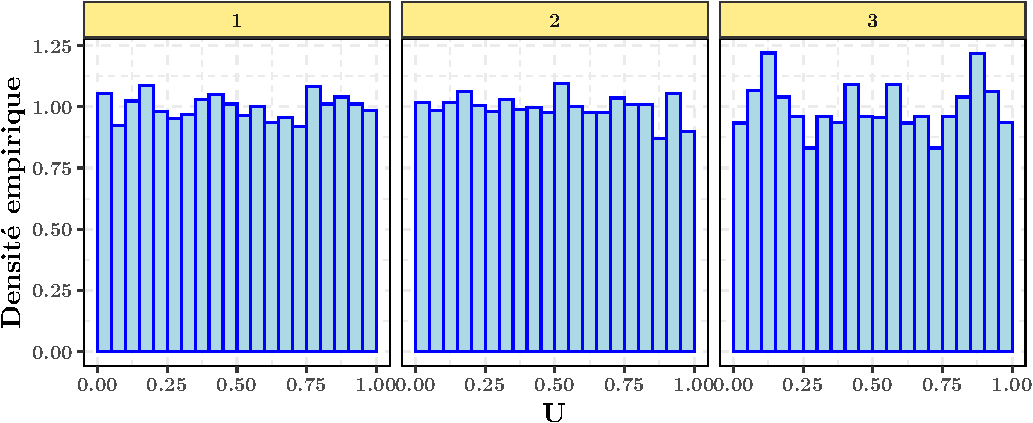
\includegraphics{diapos_simulation_variables_aleatoires_files/figure-beamer/plot_histogrammes_empiriques-1.pdf}

Au risque 5\%, avec un test de Kolmogorov-Smirnoff, on rejette

\begin{itemize}
\tightlist
\item
  \(H_0:\) Echantillon de loi uniforme \(\mathcal{U}[0, 1]\)
\end{itemize}

seulement pour l'échantillon 3.

\end{frame}

\begin{frame}{Choix important (indépendance)}
\protect\hypertarget{choix-important-induxe9pendance}{}

On regarde, pour les 3 échantillons, la valeur de \(u_k\) en fonction de
celle de \(u_{k-1}\):
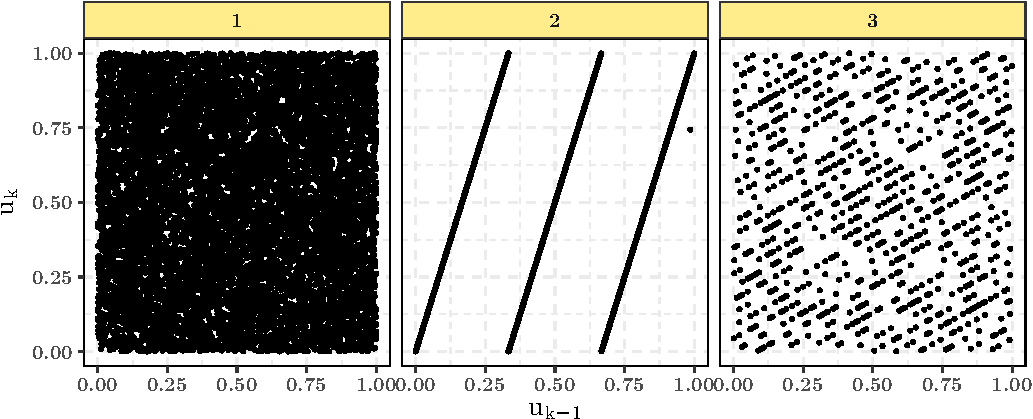
\includegraphics{diapos_simulation_variables_aleatoires_files/figure-beamer/plot_autocorrelations_empiriques-1.pdf}

Il y a une forte autocorrélation empirique dans les deux derniers
échantillons!

\end{frame}

\begin{frame}[fragile]{Loi uniforme générique}
\protect\hypertarget{loi-uniforme-guxe9nuxe9rique}{}

\begin{itemize}
\tightlist
\item
  Si on sait simuler \(U\sim \mathcal{U}[0, 1]\), alors, pour
  \(a < b \in \mathbb{R}\) \[(b - a) U + a \sim \mathcal{U}[a, b]\]
\item
  Dans \texttt{R}, la simulation d'une loi uniforme est faite avec
  \texttt{runif};
\item
  Dans la suite: on suppose qu'on sait simuler selon
  \(\mathcal{U}[0, 1]\).
\end{itemize}

\end{frame}

\hypertarget{muxe9thode-dinversion}{%
\section{Méthode d'inversion}\label{muxe9thode-dinversion}}

\begin{frame}{Rappel: Fonction de répartition}
\protect\hypertarget{rappel-fonction-de-ruxe9partition}{}

Soit \(X\) une variable aléatoire à valeurs réelles. Pour tout réel
\(x\), on appelle fonction de répartition de \(X\) la fonction \(F_X\):
\begin{align*}
\begin{array}{ccl}
\R &\mapsto& [0, 1]\\
x &\mapsto& F_X(x) = \mathbb{P}(X \leq x)
\end{array}
\end{align*}\pause Une fonction de répartition \(F_X\) est caractérisée
par les propriétés suivantes:

\begin{enumerate}
\item $F_X$ est partout continue à droite, i.e. pour tout $x\in \R$: $$\lim_{h \underset{>0}{\rightarrow} 0} F(x + h) = F(x)$$
\item $F_X$ est croissante.
\item $\lim_{x \rightarrow -\infty}F_X(x) = 0, \lim_{x \rightarrow +\infty}F_X(x) = 1$
\end{enumerate}

Ainsi, toute fonction \(F\) sur \(\R\) satisfaisant ces conditions est
une fonction de répartition.

\end{frame}

\begin{frame}{Exemple: Fonction de répartition}
\protect\hypertarget{exemple-fonction-de-ruxe9partition}{}

\begin{figure}
\centering
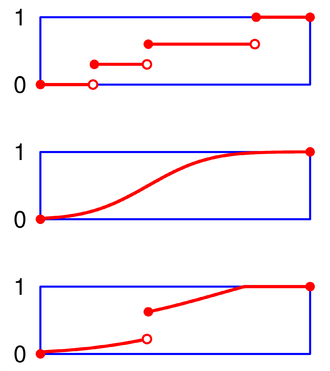
\includegraphics[height = 0.7\textheight]{figures/fonction_repartition}
\caption{\label{fig:fonc:rep} Exemples de fonction de répartition pour une variable aléatoire discrète (haut), continue (centre) ou avec atome (bas). Source \textit{Wikipedia}.}
\end{figure}

\end{frame}

\begin{frame}{Inverse généralisée de \(F\) (fonction quantile)}
\protect\hypertarget{inverse-guxe9nuxe9ralisuxe9e-de-f-fonction-quantile}{}

Soit \(F\) une fonction de répartition, on appelle inverse généralisée
de \(F\), notée, \(F^{-1}\) la fonction: \begin{align*}
\begin{array}{ccl}
]0, 1[&\mapsto& \R\\
u &\mapsto& F^{-1}(u) = \inf\left\lbrace z \in \R \text{ tel que } F(z) \geq u \right\rbrace
\end{array}
\end{align*} Pour une variable aléatoire \(X\), la fonction \(F_X^{-1}\)
est également appelée \emph{fonction quantile} de la variable aléatoire
\(X\). On convient que \(F_X^{-1}(0)\) et \(F_X^{-1}(1)\) sont la plus
petite et la plus grande des valeurs du support de \(X\) (éventuellement
infinies).

\end{frame}

\begin{frame}{Inverse généralisée}
\protect\hypertarget{inverse-guxe9nuxe9ralisuxe9e}{}

\textbf{Remarque:} Dans le cas d'une fonction de répartition \(F\)
continue et strictement croissante sur \(\R\), la fonction \(F^{-1}\)
est simplement l'inverse de \(F\).

\end{frame}

\begin{frame}{Méthode d'inversion}
\protect\hypertarget{muxe9thode-dinversion-1}{}

Supposon qu'on ait une variable aléatoire \(X\) dont on connait la
fonction de répartiion \(F\), comment simuler \(X\)?\pause

\emph{Exemple:} \(X\sim \mathcal{E}xp(\lambda)\):

\begin{itemize}
\tightlist
\item
  \textbf{Densité:}
  \(f(x) = \lambda\text{e}^{-\lambda x}\mathbf{1}_{x \geq 0}\) \pause
\item
  \textbf{Fonction de répartition: }
  \(F(x) = \int_{-\infty}^x f(z)\text{d}z = (1 - \text{e}^{-\lambda x})\mathbf{1}_{x \geq 0}\)
  \pause
\item
  \textbf{Inverse généralisée: }
  \(0<u<1,~F^{-1}(u) = -\frac{\ln (1-u)}{\lambda}\) \pause
\end{itemize}

\textbf{Méthode d'inversion} Soit \(F\) une fonction de répartition.
Soit \(F^{-1}\) son inverse généralisée. Soit \(U\) une variable
aléatoire de loi uniforme sur \([0, 1]\), alors la variable aléatoire
\[X := F^{-1}(U)\] admet \(F\) comme fonction de répartition.

\end{frame}

\begin{frame}[fragile]{Exemple de méthode d'inversion}
\protect\hypertarget{exemple-de-muxe9thode-dinversion}{}

\[F^{-1}(u) = -\frac{\ln (1-u)}{\lambda}\]

\begin{Shaded}
\begin{Highlighting}[]
\NormalTok{mon_rexp <-}\StringTok{ }\ControlFlowTok{function}\NormalTok{(n, lambda)\{}
  \CommentTok{# On simule selon une loi uniforme}
\NormalTok{  us <-}\StringTok{ }\KeywordTok{runif}\NormalTok{(n) }\CommentTok{# Echantillon IID U[0,1]}
  \CommentTok{# On applique la fonction quantile a l'échantillon}
  \OperatorTok{-}\StringTok{ }\KeywordTok{log}\NormalTok{(}\DecValTok{1} \OperatorTok{-}\StringTok{ }\NormalTok{us) }\OperatorTok{/}\StringTok{ }\NormalTok{lambda}
\NormalTok{\}}
\end{Highlighting}
\end{Shaded}

\end{frame}

\begin{frame}{Exemple de méthode d'inversion}
\protect\hypertarget{exemple-de-muxe9thode-dinversion-1}{}

\[F^{-1}(u) = -\frac{\ln (1-u)}{\lambda}\]

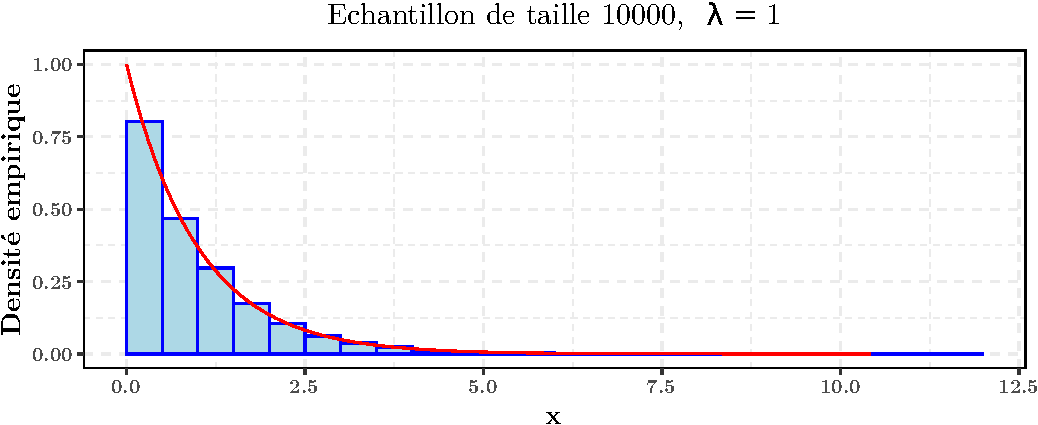
\includegraphics{diapos_simulation_variables_aleatoires_files/figure-beamer/plot_mon_rexp-1.pdf}

\end{frame}

\begin{frame}{Preuve de la méthode d'inversion}
\protect\hypertarget{preuve-de-la-muxe9thode-dinversion}{}

On veut montrer que, pour tout \(x\in \R\), si
\(U\sim \mathcal{U}[0,1]\), alors \begin{align}
\mathbb{P}(F^{-1}(U) \leq x) &= F(x).\nonumber \pause
\intertext{Montrons tout d'abord que, pour tout $u \in ]0, 1[$}
\forall x \in \R,F^{-1}(u) \leq x &\Leftrightarrow u \leq F(x). \label{eq:lemma:inv}
\end{align} \pause En effet, si on y parvient, il restera à conclure en
se servant de la définition d'une loi uniforme:
\[\mathbb{P}(F^{-1}(U) \leq x) \overset{\text{par \eqref{eq:lemma:inv}}}{=} \mathbb{P}(U \leq F(x))  \overset{\text{car }U\sim\mathcal{U}[0,1]}= F(x).\]

\end{frame}

\begin{frame}{Preuve de la méthode d'inversion}
\protect\hypertarget{preuve-de-la-muxe9thode-dinversion-1}{}

Montrons d'abord que, pour tout \(u \in ]0, 1[\) \begin{align*}
\forall x \in \R,F^{-1}(u) \leq x &\Rightarrow u \leq F(x).
\end{align*} \pause

\begin{itemize}
\item[$\Rightarrow$] Soient $u \in ]0, 1[$ et $x\in \R$ tels que $F^{-1}(u) \leq x$. \newline
Par croissance de $F$, on a donc:
\begin{align*}
F\left(F^{-1}(u)\right) &\leq F(x)
\intertext{Or, en se souvenant que par définition}
F^{-1}(u) &= \inf\left\lbrace z \in \R \text{ tel que } F(z) \geq u \right\rbrace,
\intertext{on a donc directement}
u&\leq  F\left(F^{-1}(u)\right) \leq F(x)
\end{align*}
\end{itemize}

\end{frame}

\begin{frame}{Preuve de la méthode d'inversion}
\protect\hypertarget{preuve-de-la-muxe9thode-dinversion-2}{}

Montrons maintenant, pour tout \(u \in ]0, 1[\) \begin{align*}
\forall x \in \R,F^{-1}(u) \leq x &\Leftarrow u \leq F(x).
\end{align*}\pause

\begin{itemize}
\item[$\Leftarrow$] Soient $u \in ]0, 1[$ et $x\in \R$ tels que $u \leq F(x)$.\newline
Ainsi, $x\in\left\lbrace z \in \R \text{ tel que } F(z) \geq u \right\rbrace$, donc $F^{-1}(u) \leq x$.
\end{itemize}

\end{frame}

\begin{frame}{Intérêt de la méthode d'inversion}
\protect\hypertarget{intuxe9ruxeat-de-la-muxe9thode-dinversion}{}

Ainsi, pour une variable aléatoire à valeurs dans \(\mathbb{R}\), on
sait simuler si on connaît l'inverse généralisée de sa fonction de
répartition.

\end{frame}

\hypertarget{muxe9thode-dacceptation-rejet}{%
\section{Méthode d'acceptation
rejet}\label{muxe9thode-dacceptation-rejet}}

\begin{frame}{Exemple motivant}
\protect\hypertarget{exemple-motivant}{}

On veut simuler selon la densité
\(f(x) = \sqrt{\frac{2}{\pi}}\text{e}^{-\frac{x^2}{2}}\mathbf{1}_{x \geq 0}\).

La fonction quantile n'a pas d'expression analytique. La méthode
d'inversion ne peut être appliquée.\pause

\textbf{Principe de la méthode d'acceptation rejet:}

\begin{itemize}
\tightlist
\item
  Simuler des \emph{candidats} selon une autre loi qu'on sait simuler.
  \pause 
\item
  Choisir parmi les candidats grâce à la loi uniforme.
\end{itemize}

\end{frame}

\begin{frame}{Méthode d'acceptation rejet (proposition)}
\protect\hypertarget{muxe9thode-dacceptation-rejet-proposition}{}

Soit \(f\) et \(g\) deux densités sur \(\R^d\). On suppose qu'il existe
une constante \(M\) telle que \[\forall x \in \R^d~~f(x) \leq M g(x)\]
On note \[0 \leq r(x) := \frac{f(x)}{Mg(x)} \leq 1.\] \pause -Soient
\((Y_n)_{n\geq 1}\) une suite de variables aléatoires i.i.d. de densité
\(g\) et \((U_n)_{n\geq 1}\) une suite de variables aléatoires i.i.d. de
loi uniforme sur \([0, 1]\). \pause - On note \(T\) la variable
aléatoire (à valeurs dans \(\mathbb{N}^*\)):
\[T = \inf\left\lbrace n, \text{ tel que } U_n \leq r(Y_n)\right\rbrace.\].
\pause - Alors, la variable aléatoire \(X := Y_T\) (\(T\)-ième valeur de
la suite \((Y_n)_{n\geq 1}\)) a pour densité \(f\).

\end{frame}

\begin{frame}[fragile]{Méthode d'acceptation rejet (algorithme)}
\protect\hypertarget{muxe9thode-dacceptation-rejet-algorithme}{}

On veut tirer un échantillon \(X\) de densité \(f\). On ne sait simuler
que selon la densité \(g\). On suppose qu'il existe une constante \(M\)
telle que \[\forall x \in \R^d~~f(x) \leq M g(x)\]

\textbf{Algorithme} \texttt{Condition\ \textless{}-\ FALSE}

\begin{itemize}
\tightlist
\item
  Tant que \texttt{not\ Condition}:

  \begin{itemize}
  \tightlist
  \item
    Tirer \(Y \sim g(y)\);
  \item
    Tirer (indépendemment) \(U\sim \mathcal{U}[0, 1]\);
  \item
    Si \[U \leq \frac{f(Y)}{Mg(Y)},\] alors on pose
    \texttt{Condition\ \textless{}-\ TRUE} et \(X = Y\)
  \item
    Sinon \texttt{Condition\ \textless{}-\ FALSE}
  \end{itemize}
\end{itemize}

En sortie, \(X\sim f(x)\).

\end{frame}

\begin{frame}{Méthode d'acceptation rejet: Exemple}
\protect\hypertarget{muxe9thode-dacceptation-rejet-exemple}{}

\begin{itemize}
\tightlist
\item
  On veut simuler selon
  \(f(x) = \sqrt{\frac{2}{\pi}}\text{e}^{-\frac{x^2}{2}}\mathbf{1}_{x \geq 0}\)
\item
  On considère \(g(x) = \text{e}^{-x}\mathbf{1}_{x \geq 0}\) (densité
  d'un \(\mathcal{E}xp(\lambda = 1) )\)\\
\item
  On montre que
  \[\forall x \in \R,~f(x) \leq \overbrace{\sqrt{\frac{2}{\pi}} \text{e}^{\frac{1}{2}}}^Mg(x)\]
\end{itemize}

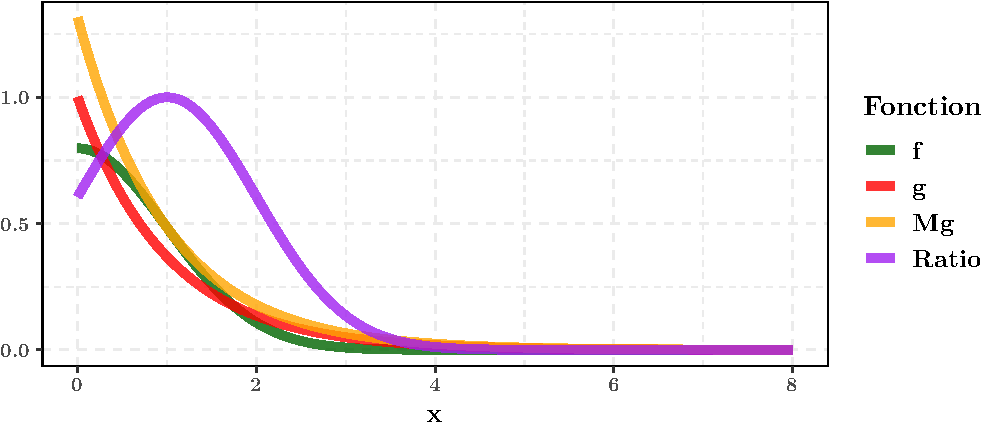
\includegraphics{diapos_simulation_variables_aleatoires_files/figure-beamer/plot_function-1.pdf}

\end{frame}

\begin{frame}{Méthode d'acceptation rejet: Exemple}
\protect\hypertarget{muxe9thode-dacceptation-rejet-exemple-1}{}

\begin{itemize}
\tightlist
\item
  On simule 10000 points selon \(g\)
\end{itemize}

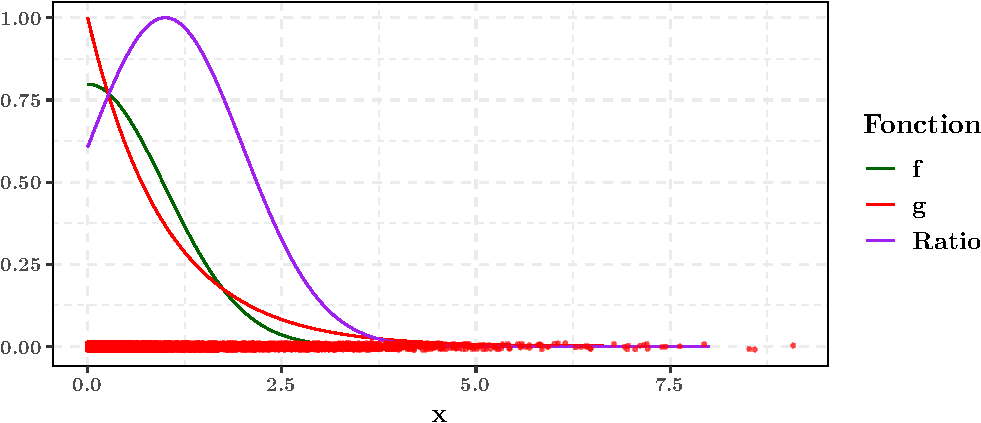
\includegraphics{diapos_simulation_variables_aleatoires_files/figure-beamer/plot_simulated-1.pdf}

\end{frame}

\begin{frame}{Méthode d'acceptation rejet: Exemple}
\protect\hypertarget{muxe9thode-dacceptation-rejet-exemple-2}{}

\begin{itemize}
\tightlist
\item
  On simule 10000 points selon \(g\)
\item
  On accepte avec une probabilité donnée par le ratio
\end{itemize}

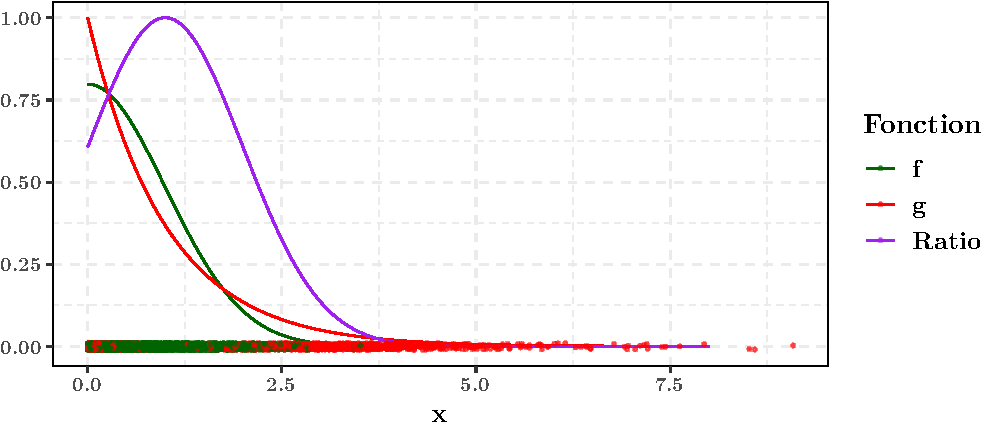
\includegraphics{diapos_simulation_variables_aleatoires_files/figure-beamer/plot_simulated_accepted-1.pdf}

\end{frame}

\begin{frame}{Méthode d'acceptation rejet: Exemple}
\protect\hypertarget{muxe9thode-dacceptation-rejet-exemple-3}{}

\begin{itemize}
\tightlist
\item
  On simule 10000 points selon \(g\)
\item
  On accepte avec une probabilité donnée par le ratio
\item
  Les points acceptés sont i.i.d. de densité \(f\).
\end{itemize}

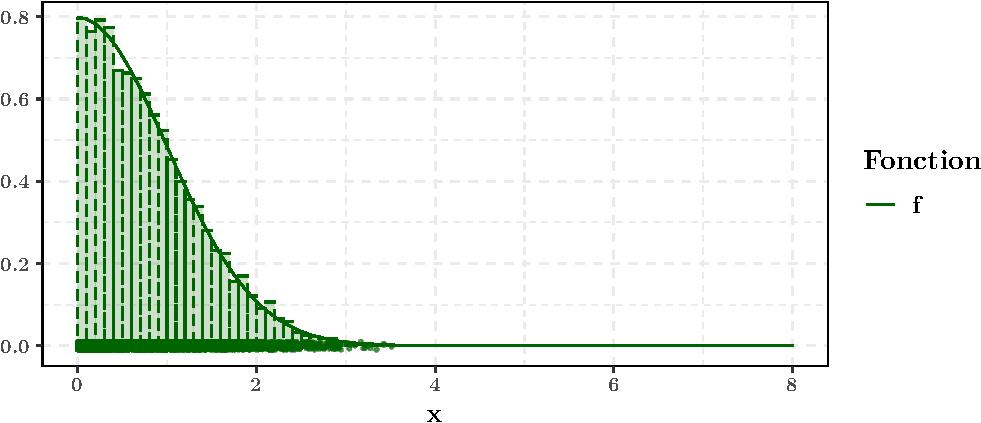
\includegraphics{diapos_simulation_variables_aleatoires_files/figure-beamer/plot_simulated_plus_histo-1.pdf}

\end{frame}

\begin{frame}{Remarque}
\protect\hypertarget{remarque}{}

Sur l'exemple précédent, au lieu de faire un ``tant que'', on a simuler
10000 points et on n'a retenu que les acceptés. \pause

\begin{itemize}
\tightlist
\item
  Proportion empirique acceptée: 0.761
\item
  D'un autre côté, on a \(1/M = 0.76\)
\end{itemize}

\end{frame}

\begin{frame}{Preuve de la méthode d'acceptation rejet}
\protect\hypertarget{preuve-de-la-muxe9thode-dacceptation-rejet}{}

Preuve à connaître!

\begin{itemize}
\tightlist
\item
  Voir le poly de cours.
\item
  Analogue de la preuve sera demandée en devoir.
\end{itemize}

\end{frame}

\begin{frame}[fragile]{Code R}
\protect\hypertarget{code-r}{}

\begin{Shaded}
\begin{Highlighting}[]
\NormalTok{get_one_sample <-}\StringTok{ }\ControlFlowTok{function}\NormalTok{()\{}
\NormalTok{  condition <-}\StringTok{ }\OtherTok{FALSE}
  \ControlFlowTok{while}\NormalTok{(}\OperatorTok{!}\NormalTok{condition)\{}
\NormalTok{    y <-}\StringTok{ }\KeywordTok{simulate_g}\NormalTok{(...) }\CommentTok{# Simulation selon g}
\NormalTok{    u <-}\StringTok{ }\KeywordTok{runif}\NormalTok{(}\DecValTok{1}\NormalTok{) }\CommentTok{# Uniform}
    \CommentTok{# On suppose que f, g, et M existent}
\NormalTok{    condition <-}\StringTok{ }\NormalTok{u }\OperatorTok{<=}\StringTok{ }\KeywordTok{f}\NormalTok{(y) }\OperatorTok{/}\StringTok{ }\NormalTok{(M }\OperatorTok{*}\StringTok{ }\KeywordTok{g}\NormalTok{(y))}
\NormalTok{  \}}
  \KeywordTok{return}\NormalTok{(y)}
\NormalTok{\}}
\end{Highlighting}
\end{Shaded}

\end{frame}

\begin{frame}{Loi du temps d'attente}
\protect\hypertarget{loi-du-temps-dattente}{}

On s'arrête au premier temps tel qu'une uniforme est inférieure au ratio
observée.

La loi du temps d'attente (voir preuve) est une \textbf{loi géométrique}
sur \(\mathbb{N}^*\) de paramètre \(\frac{1}{M}\) .

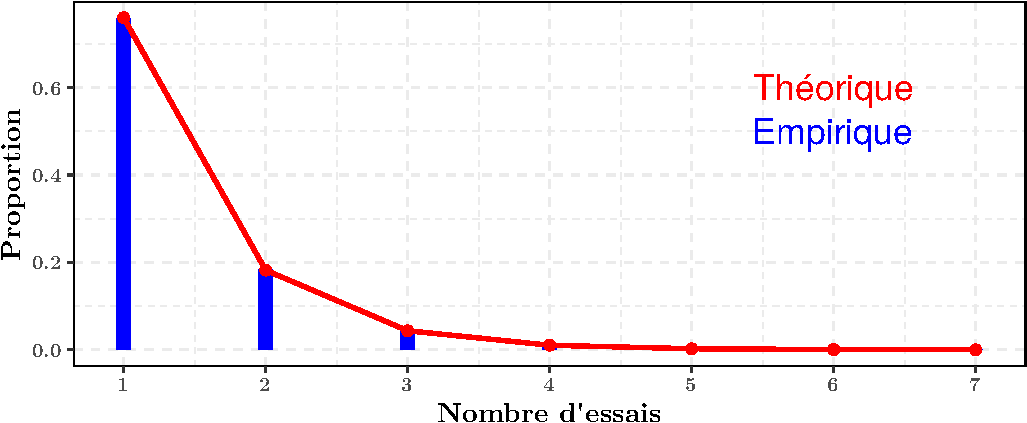
\includegraphics{diapos_simulation_variables_aleatoires_files/figure-beamer/plot_temps_attente-1.pdf}

\end{frame}

\begin{frame}{Vecteurs aléatoires}
\protect\hypertarget{vecteurs-aluxe9atoires}{}

Pour simuler un vecteur aléatoire \((X, Y)\), on pourra utiliser (voir
poly et TD pour des exemples):

\begin{itemize}
\tightlist
\item
  Conditionnement;
\item
  Changement de variables
\end{itemize}

\end{frame}

\begin{frame}{Changements de variables pour densité}
\protect\hypertarget{changements-de-variables-pour-densituxe9}{}

Soit un couple de variables aléatoires \((U,V)\) de densité
\(f_{U,V}(u,v)\) définie sur \(E_{UV} \subset \R^2\) et un couple de
variables aléatoires \((X, Y)\) à valeurs dans \(E_{XY} \subset \R^2\).
Supposons qu'il existe une application \(\phi\), \(C^1\), inversible, et
d'inverse \(C^1\), tel que \((X, Y) = \phi(U, V)\), alors la densité
jointe de \((X, Y)\) est donnée par:
\[f_{X,Y}(x, y) = f_{U,V}(\phi^{-1}(x, y))\vert\det J_{\phi^{-1}}(x, y)\vert  \]
où \(J_\phi\) désigne la matrice jacobienne d'une application
\(\phi(u, v)\): \[J_\phi(u, v) = \begin{pmatrix}
\frac{\delta \phi_1}{\delta u}(u, v) & \frac{\delta \phi_1}{\delta v}(u, v)\\
\frac{\delta \phi_2}{\delta u}(u, v) & \frac{\delta \phi_2}{\delta v}(u, v)
\end{pmatrix}\]

\end{frame}

\end{document}
